% !TeX spellcheck = en_US
\documentclass[]{scrartcl}

\usepackage{graphicx}
\usepackage{amsmath}
\usepackage{hyperref}

%opening
\title{Lab 2}
\author{}

\begin{document}

\maketitle

\begin{abstract}

\end{abstract}

\section{Spectral analysis of a synthetic signal}

\subsection{R1.a),R1.b) Synthetic signal}\label{sec:R1a}
First of all, the signal $x(n)$ of duration $M=512$ was created, as given by 
\begin{equation}\label{eq:defx}
	x(n) = 5\cos(\omega_0 n +1)+2\cos(2\omega_0 n +2)+3\cos(5\omega_0 n +3)\:,
\end{equation}
with $\omega_0 = 5.2\times 2\pi/M$ rad. The signal $x(n)$ is presented in Fig. \ref{fig:R1b}. As it is possible to observe from \eqref{eq:defx} and Fig. \ref{fig:R1b}, the signal $x(n)$ is composed of a linear combination three harmonics, whose frequency are integer which are multiples of the lowest frequency $\omega_0$. Note that such angular frequency can be written as a rational fraction of $2\pi$ as $\omega_0 = 2\pi \times 13/1280$.
\begin{figure}[htbp]
	\centering
	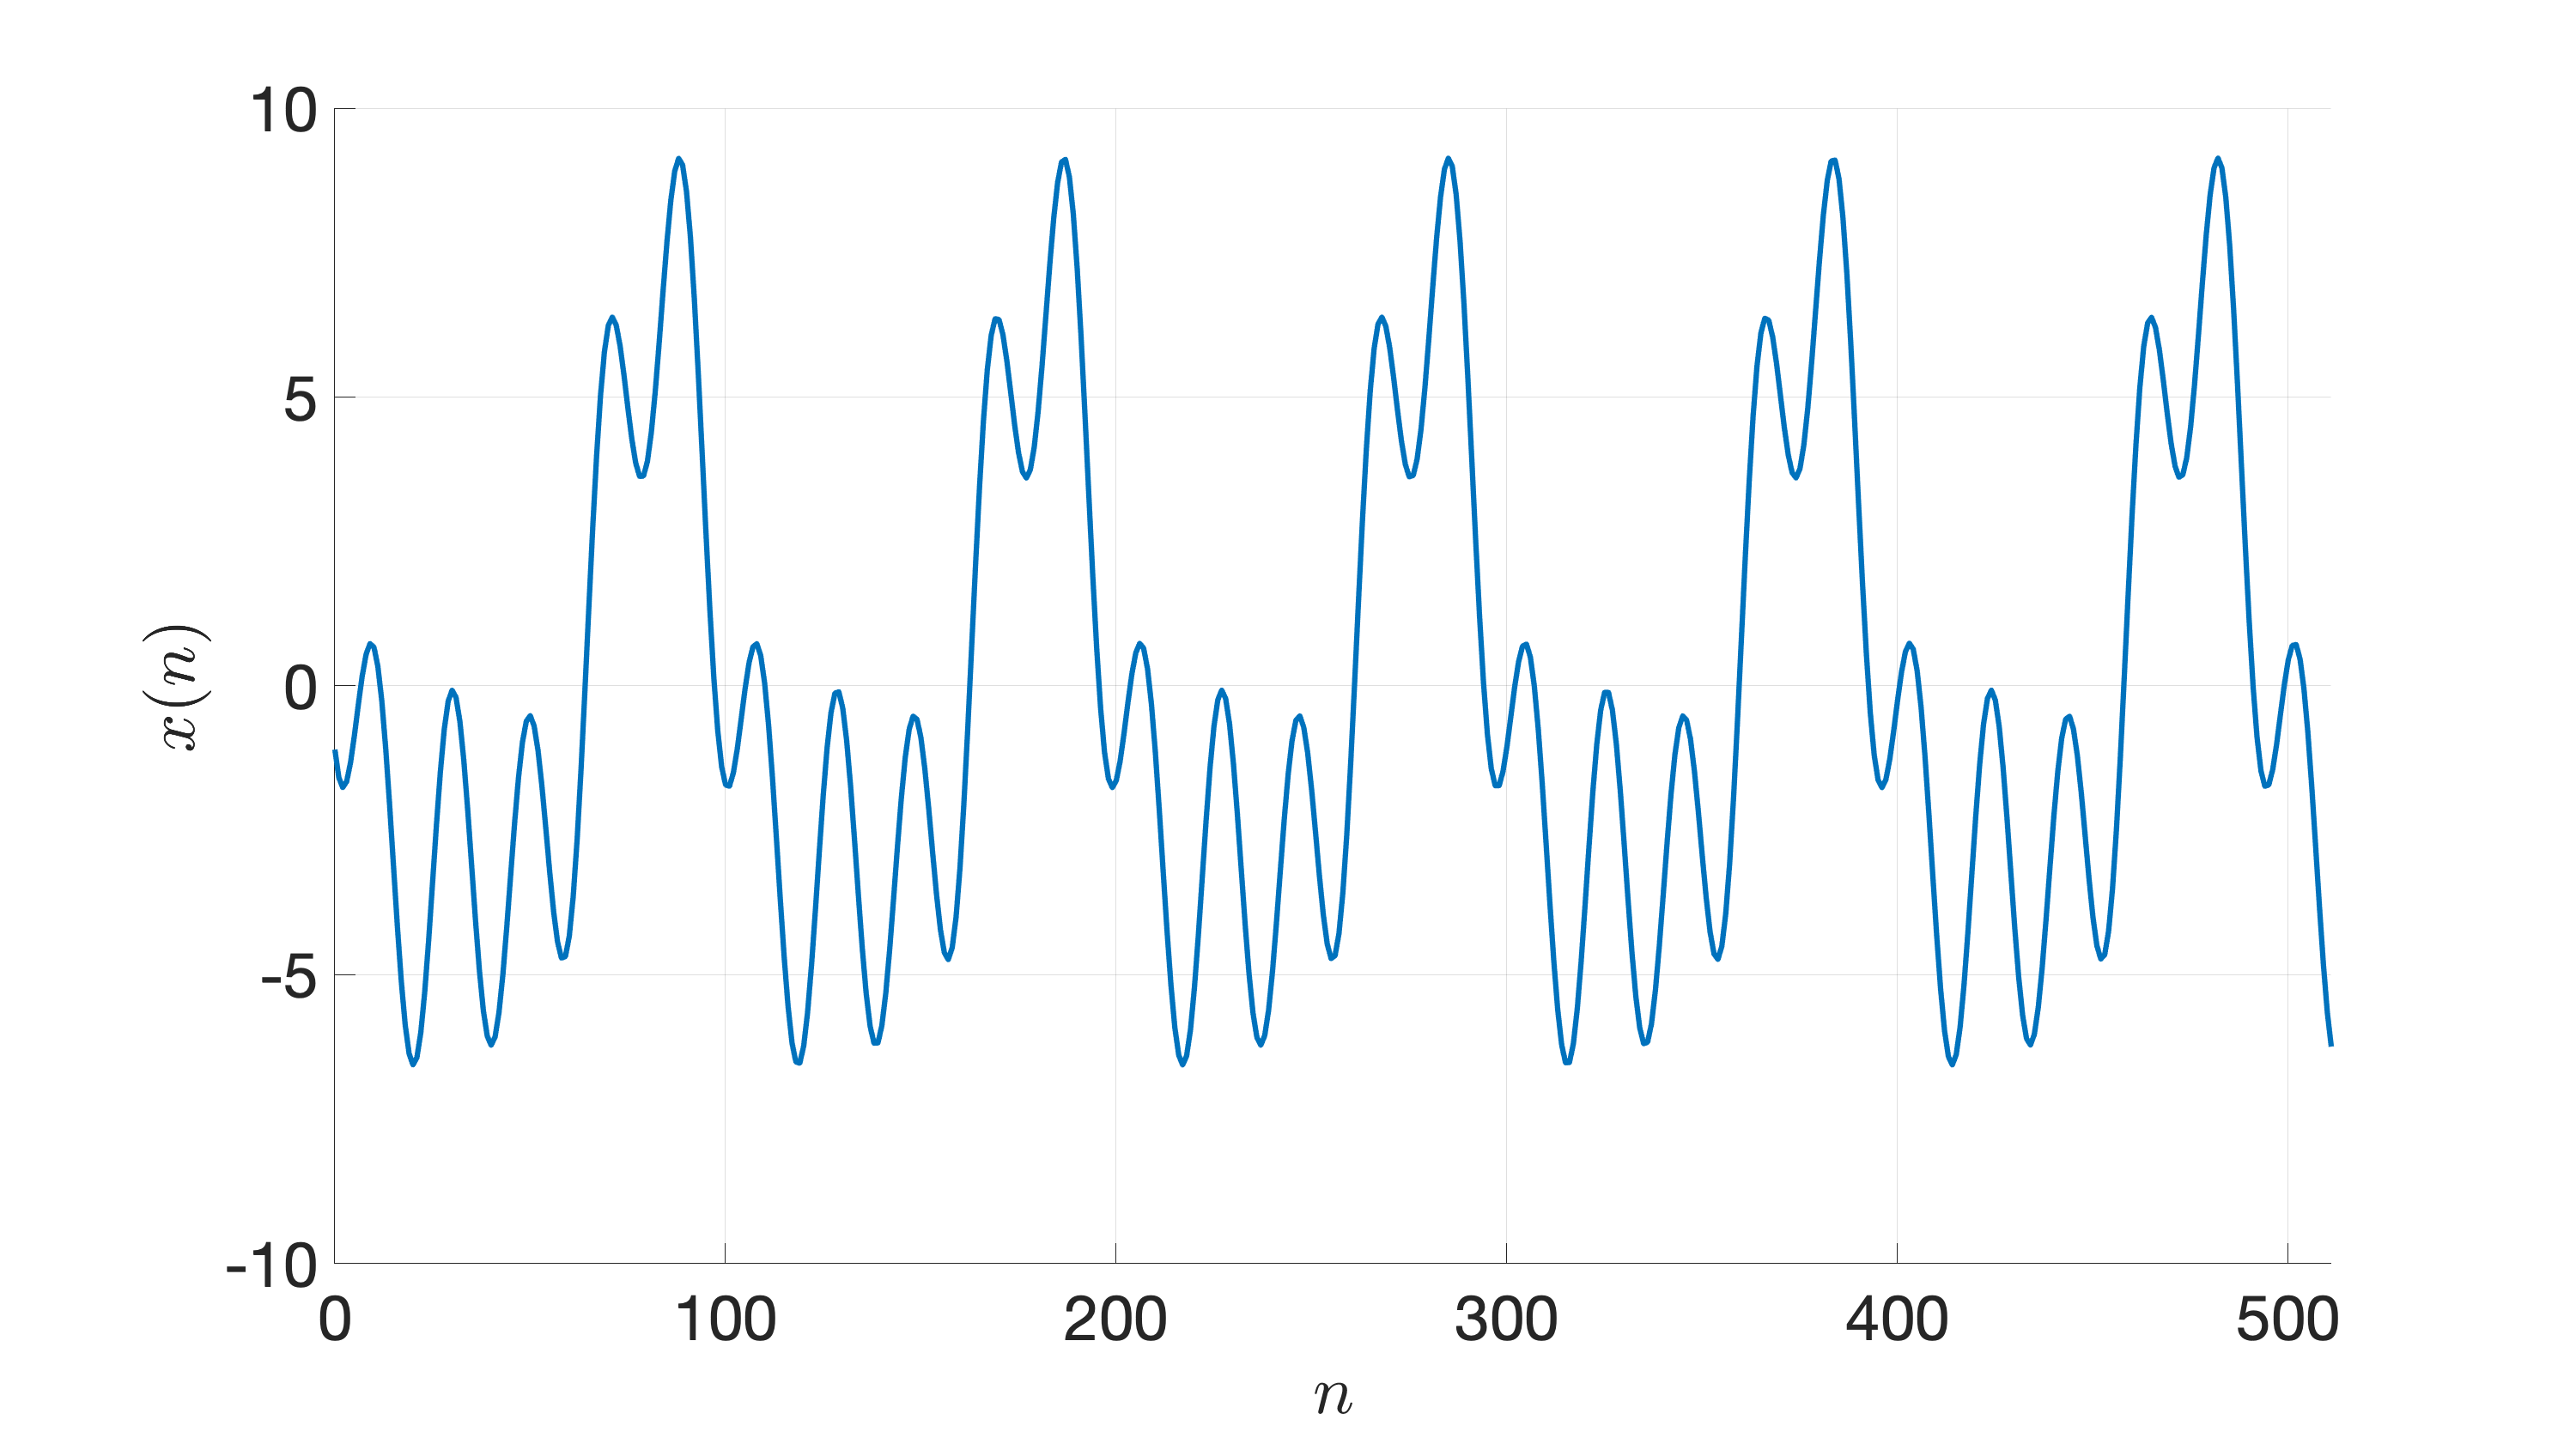
\includegraphics[width= 0.8\textwidth]{figures/R1b.png}
	\caption{Synthetic signal.}
	\label{fig:R1b}
\end{figure}

\subsection{R1.c) Discrete Fourier Transform}

Second of all, the one-sided Discrete Fourier Transform (DFT) of length $N= 512$ of signal $x(n)$ was computed. Figs. \ref{fig:R1c_mag} and \ref{fig:R1c_arg} show the magintude and phase of the one-sided DFT coefficients $X(k)$, repectively, in function of the normalized frequency $\omega = 2\pi k/N$. It is evident that there are 3 peaks of the magnitude of the DFT, each corresponding to an harmonic of signal $x(n)$, as expected.

\begin{figure}[htbp]
	\centering
	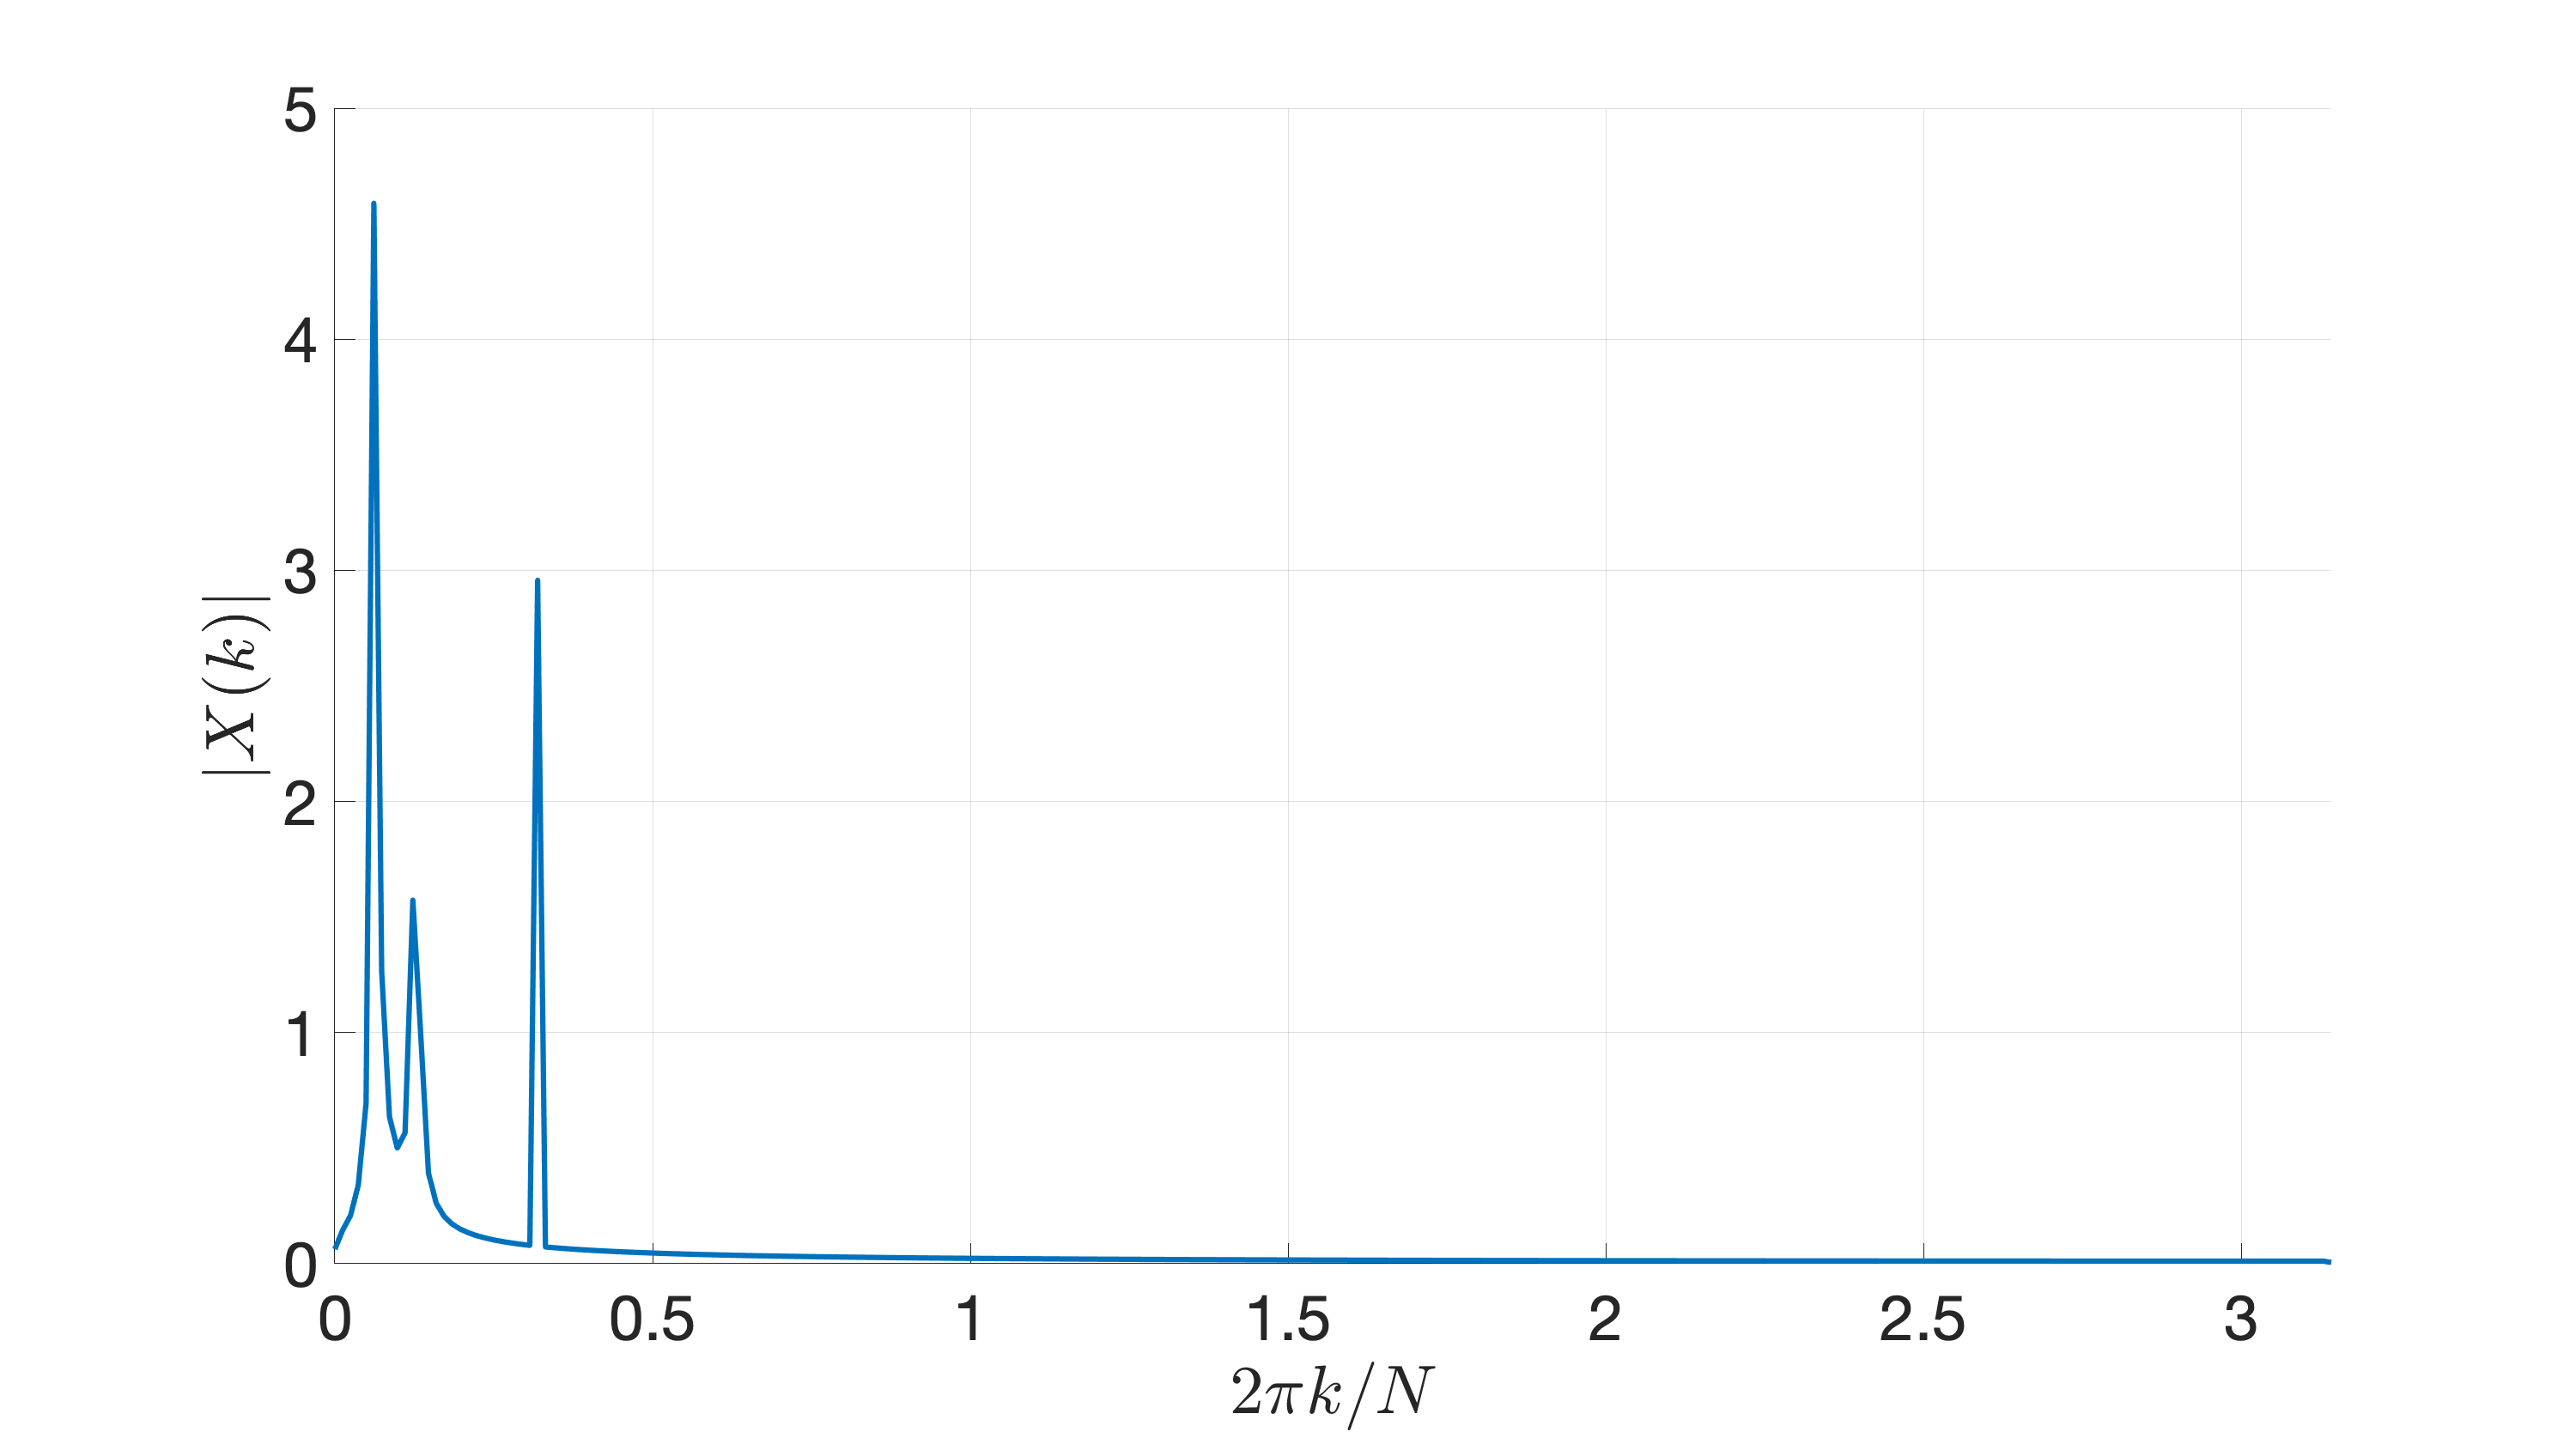
\includegraphics[width= 0.8\textwidth]{figures/R1c_mag.png}
	\caption{Magnitude of the one-sided DFT coefficients as a function of the normalized frequency.}
	\label{fig:R1c_mag}
\end{figure}
\begin{figure}[htbp]
	\centering
	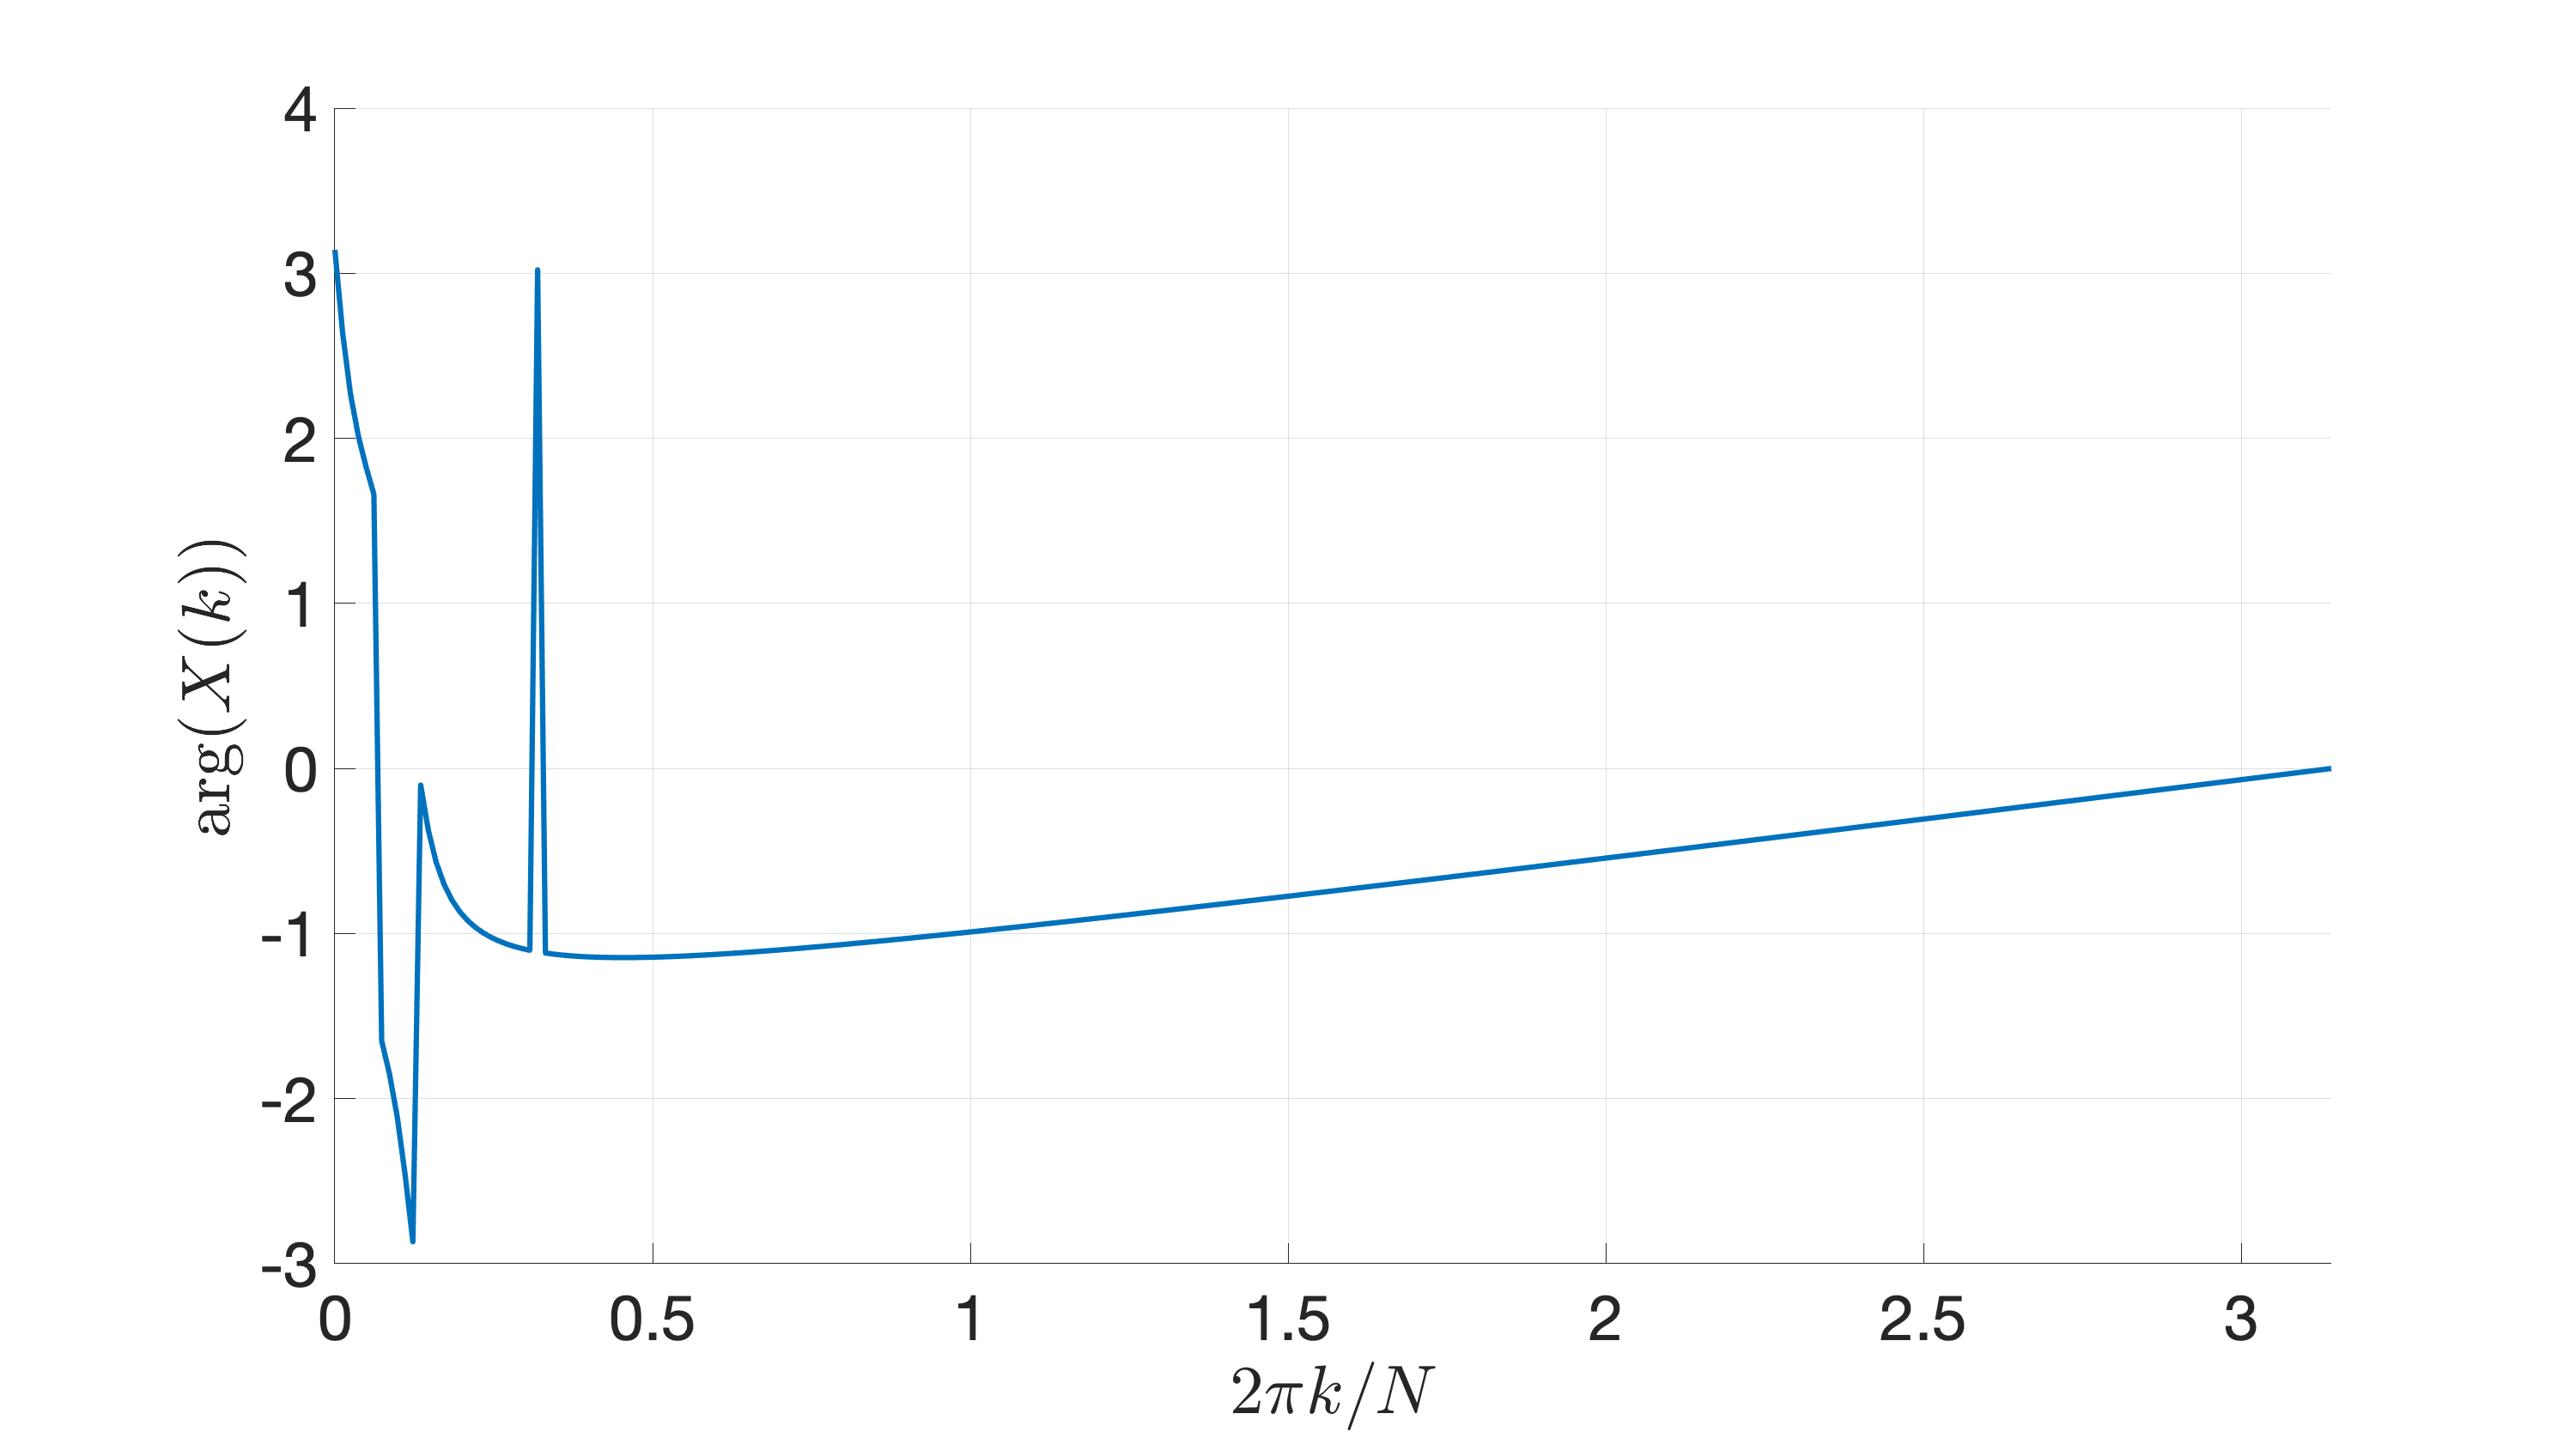
\includegraphics[width= 0.8\textwidth]{figures/R1c_arg.png}
	\caption{Argument of the one-sided DFT coefficients as a function of the normalized frequency.}
	\label{fig:R1c_arg}
\end{figure}

\subsection{R1.d) Peaks of the magnitude of the DFT coefficients}
The index $k$, normalized frequency $\omega(k)$, magnitude $|X(k)|$, and argument $\mathrm{arg}(|X(k)|)$ of one-sided DFT coefficients corresponding to the peaks of Fig. \ref{fig:R1c_mag} are shown in Table \ref{tb:peaks}.

\begin{table}[htbp]
	\centering
	\caption{One-sided DFT coefficients corresponding to the peaks of Fig.\ref{fig:R1c_mag}.}
	\label{tb:peaks}
	\begin{tabular}{cccc}
		\hline
		$k$ & $\omega(k) \: (\mathrm{rad\:s^{-1}})$ & $|X(k)|$ & $\mathrm{arg}(|X(k)|)\: (\mathrm{rad})$\\
		\hline
		5 & $2\pi k/N \approx 0.0614$ & $ 4.5886$ & 1.6611\\
		10 & $2\pi k/N \approx 0.1227$ & $ 1.5735$ & -2.8673  \\
		26  & $2\pi k/N \approx 0.3191$ & $ 2.9577$ & 3.0211 \\
		\hline
	\end{tabular}
\end{table}

It is important to remark that none of the the two lowest frequency harmonics of the original signal $x(n)$ are an integer multiple of $2\pi /N$. As a result, the normalized frequencies of the corresponding peaks of the one-sided DFT do not exactly correspond to the frequencies of the harmonics of the original signal. On the other hand, the frequency of the third harmonic $5\omega_0$ can be written as $26\times2\pi/N$, thus the normalized frequency of the peak should match the frequency of the harmonic. Furthermore, albeit not exactly equal, the normalized frequencies, magnitude, and argument of the one-sided DFT coefficients are very close to those of the harmonics of the original signal, as it can be seen in Table \ref{tb:comp_peaks}. The closest, as expected, is the highest frequency harmonic.

\begin{table}[htbp]
	\centering
	\caption{One-sided DFT coefficients corresponding to the peaks of Fig.\ref{fig:R1c_mag}.}
	\label{tb:comp_peaks}
	\begin{tabular}{cc|cc|cc}
		\hline
		 $\omega$ & $\omega(k) \: (\mathrm{rad\:s^{-1}})$ & Amplitude & $|X(k)|$ & Phase & $\mathrm{arg}(|X(k)|)\: (\mathrm{rad})$\\
		\hline
		$\omega_0 \approx 0.0638$  & $2\pi k/N \approx 0.0614$ & 5 & $ 4.5886$ & 1 & 1.6611\\
		$2\omega_0 \approx 0.1276$ & $2\pi k/N \approx 0.1227$ & 2 & $ 1.5735$ & 2 & -2.8673  \\
		$5\omega_0 \approx 0.3191$ & $2\pi k/N \approx 0.3191$ & 3 & $ 2.9577$ & 3 & 3.0211 \\
		\hline
	\end{tabular}
\end{table}


\subsection{R1.e) Reconstruction of synthetic signal (N = 512)}

Third of all, the signal $x(n)$ can be reconstructed from the three peaks identified in one-sided magnitude spectrum, as the linear combination of complex exponential functions. The reconstructed signal $x_r(n)$ is shown and compared with the original signal in \ref{fig:R1e}. It is visible that, although it accurate in the frequency domain, it is not able to reproduce the original signal very accurately in the time domain. The sum of the squared errors amounts to $SSE \approx 1224.5$.

\begin{figure}[htbp]
	\centering
	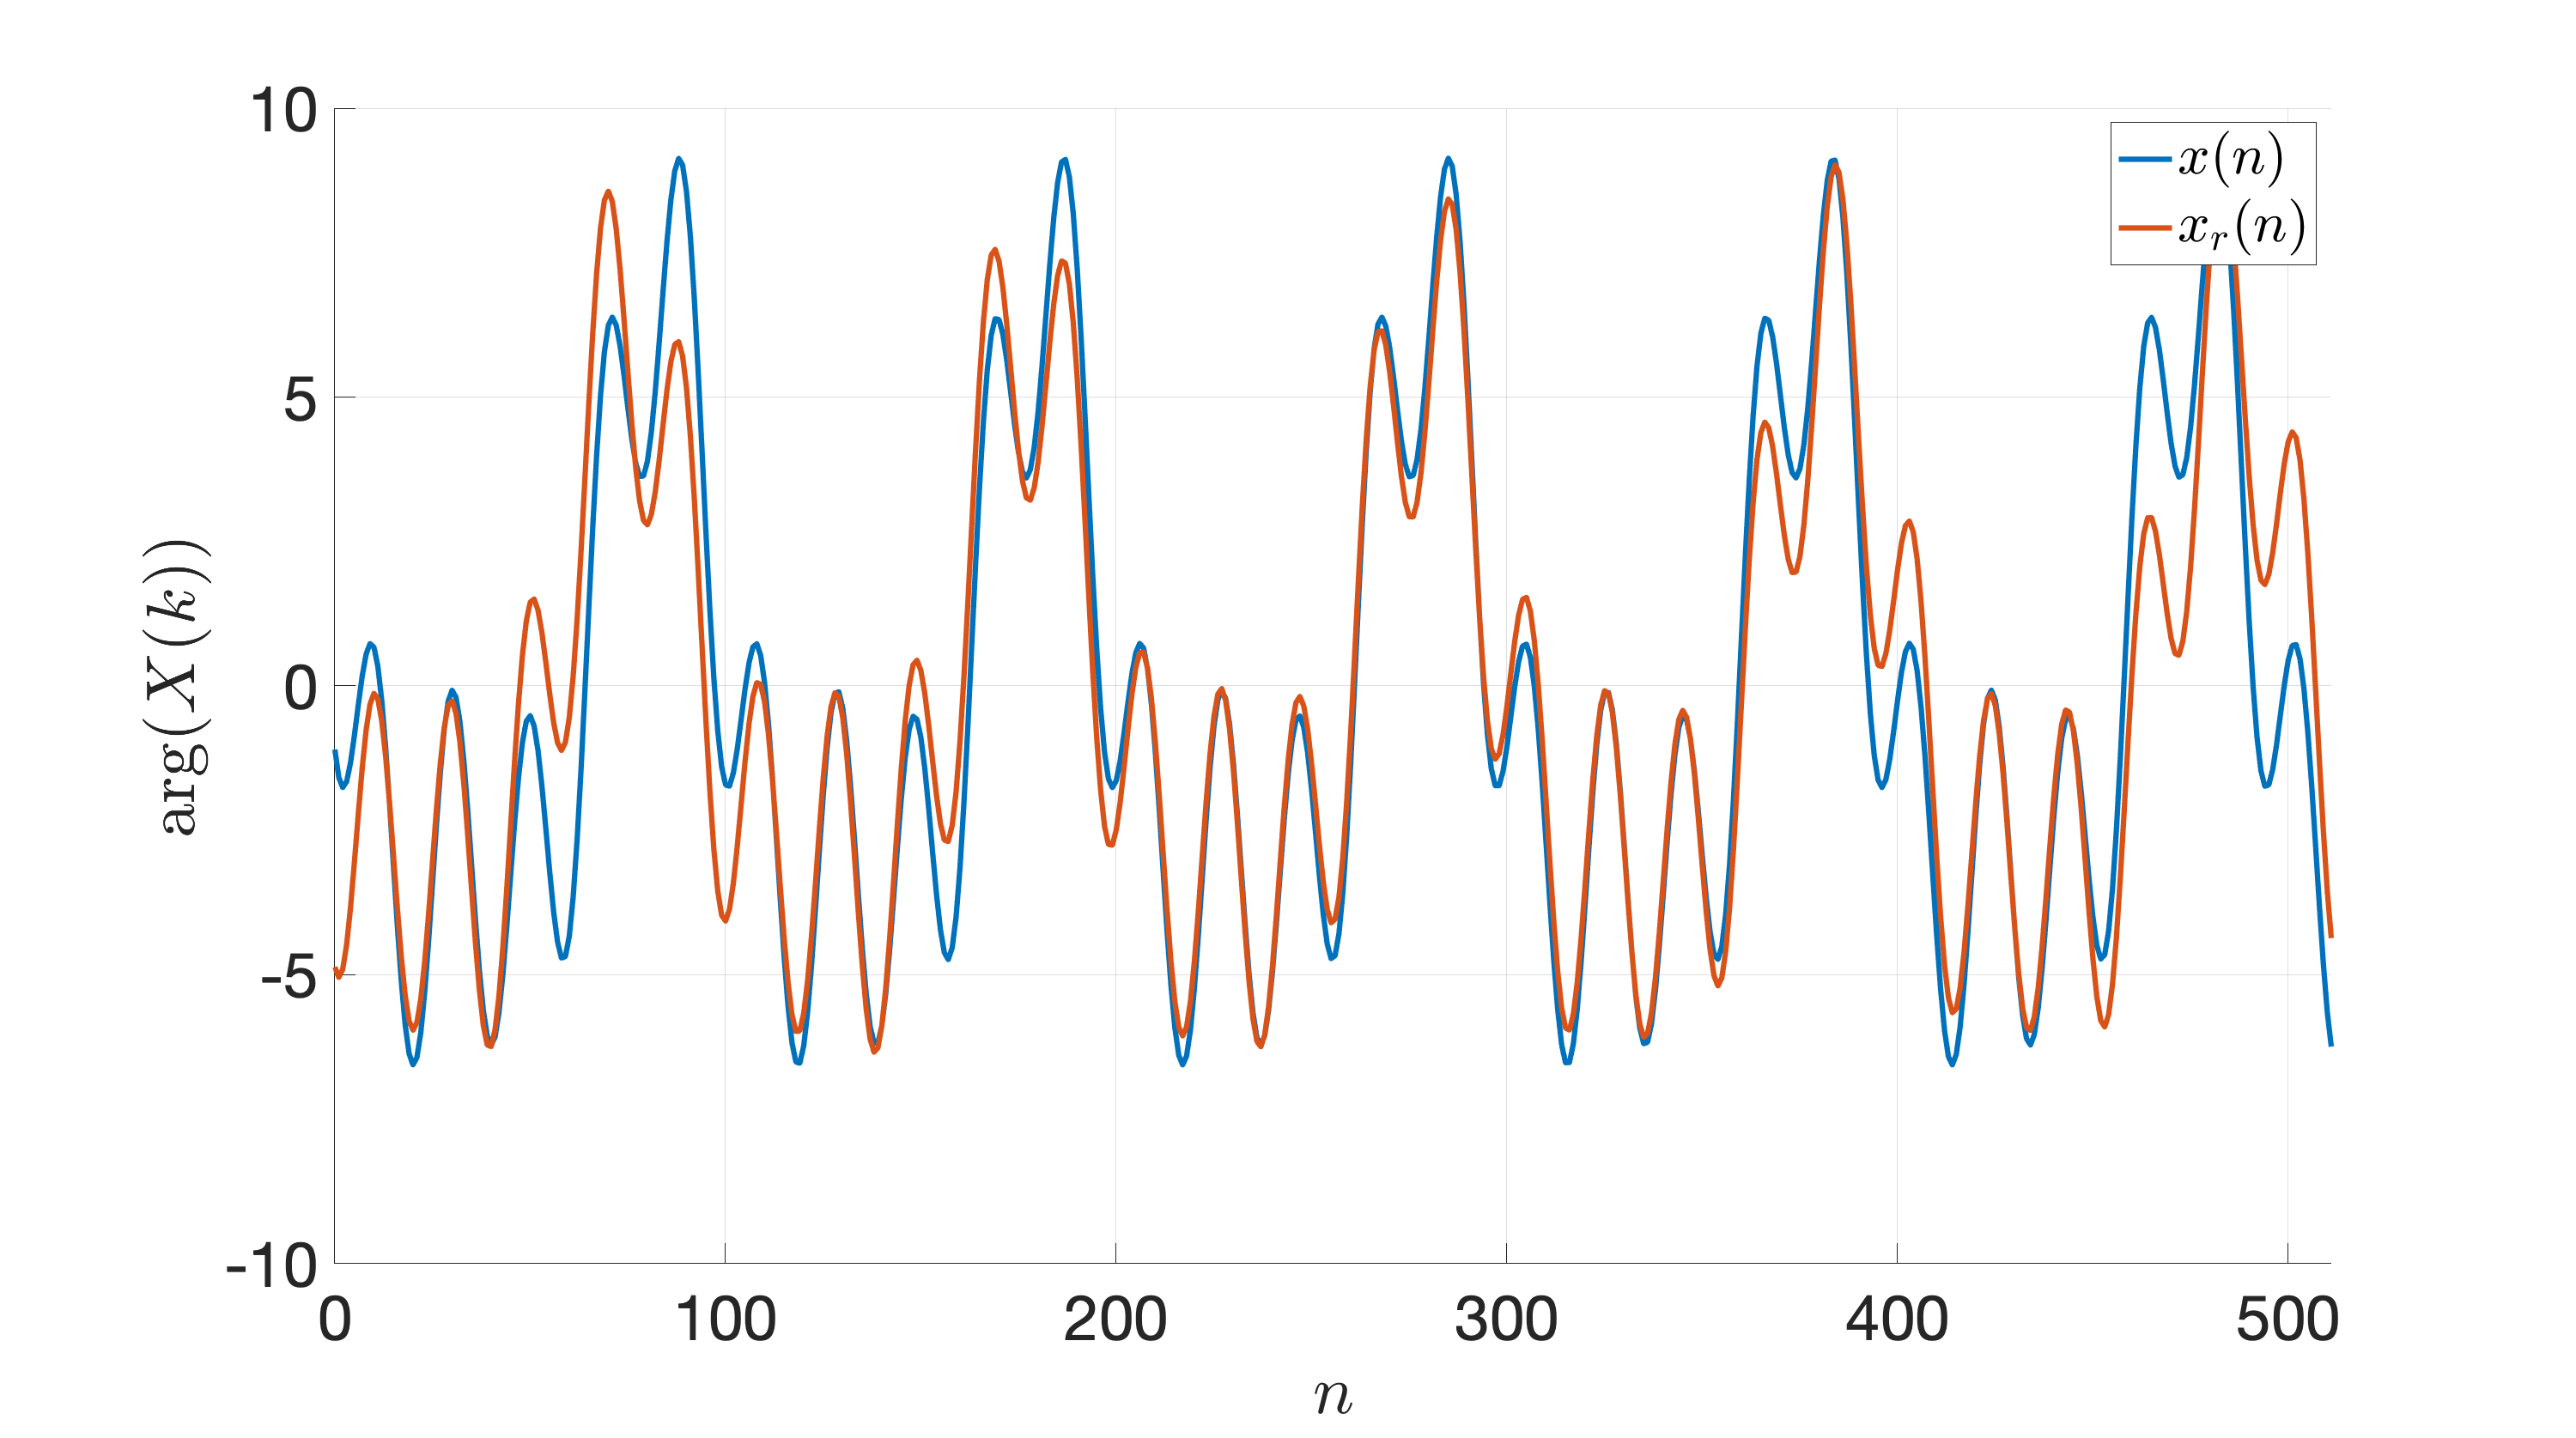
\includegraphics[width= 0.8\textwidth]{figures/R1e.png}
	\caption{Comparison between the reconstructed signal and the original, for $N = 512$.}
	\label{fig:R1e}
\end{figure}

\subsection{R1.f) Reconstruction of synthetic signal (N = 1024)}

Fourth of all, the DFT the original signal was performed with a window length of $N= 1024$. The increase of the DFT length allows to have double the precision on the normalized frequencies in relation to $N = 512$. As a result the three largest peaks identified in the one-sided magnitude spectrum of the DFT are presented in Table \ref{tb:peaks_N}. Note that, only the harmonic of frequency $2\omega_0$ as identified with more precision, as the increase of precision is not great enough to notice an improvement in the lowest frequency harmonic.

\begin{table}[htbp]
	\centering
	\caption{One-sided DFT coefficients, with $N = 1024$, corresponding to the three largest peaks of the magnitude spectrum.}
	\label{tb:peaks_N}
	\begin{tabular}{cccc}
		\hline
		$k$ & $\omega(k) \: (\mathrm{rad\:s^{-1}})$ & $|X(k)|$ & $\mathrm{arg}(|X(k)|)\: (\mathrm{rad})$\\
		\hline
		10 & $2\pi k/N \approx 0.0614$ & $ 4.5886$ & 1.6611\\
		21 & $2\pi k/N \approx 0.1289$ & $ 1.5735$ & 1.6176 \\
		52  & $2\pi k/N \approx 0.3191$ & $ 2.9577$ & 3.0211 \\
		\hline
	\end{tabular}
\end{table}


The signal $x(n)$ can, again, be reconstructed from the three peaks identified in one-sided magnitude spectrum, as the linear combination of complex exponential functions. The reconstructed signal $x_r(n)$ is shown and compared with the original signal in \ref{fig:R1f}. Comparing Figs. \ref{fig:R1e} and \ref{fig:R1f}, it is visible that it is able to reproduce the original signal more accurately. In fact, the sum of the squared errors amounts to $SSE \approx 876.5$, which is a decrease of 28\% .

\begin{figure}[htbp]
	\centering
	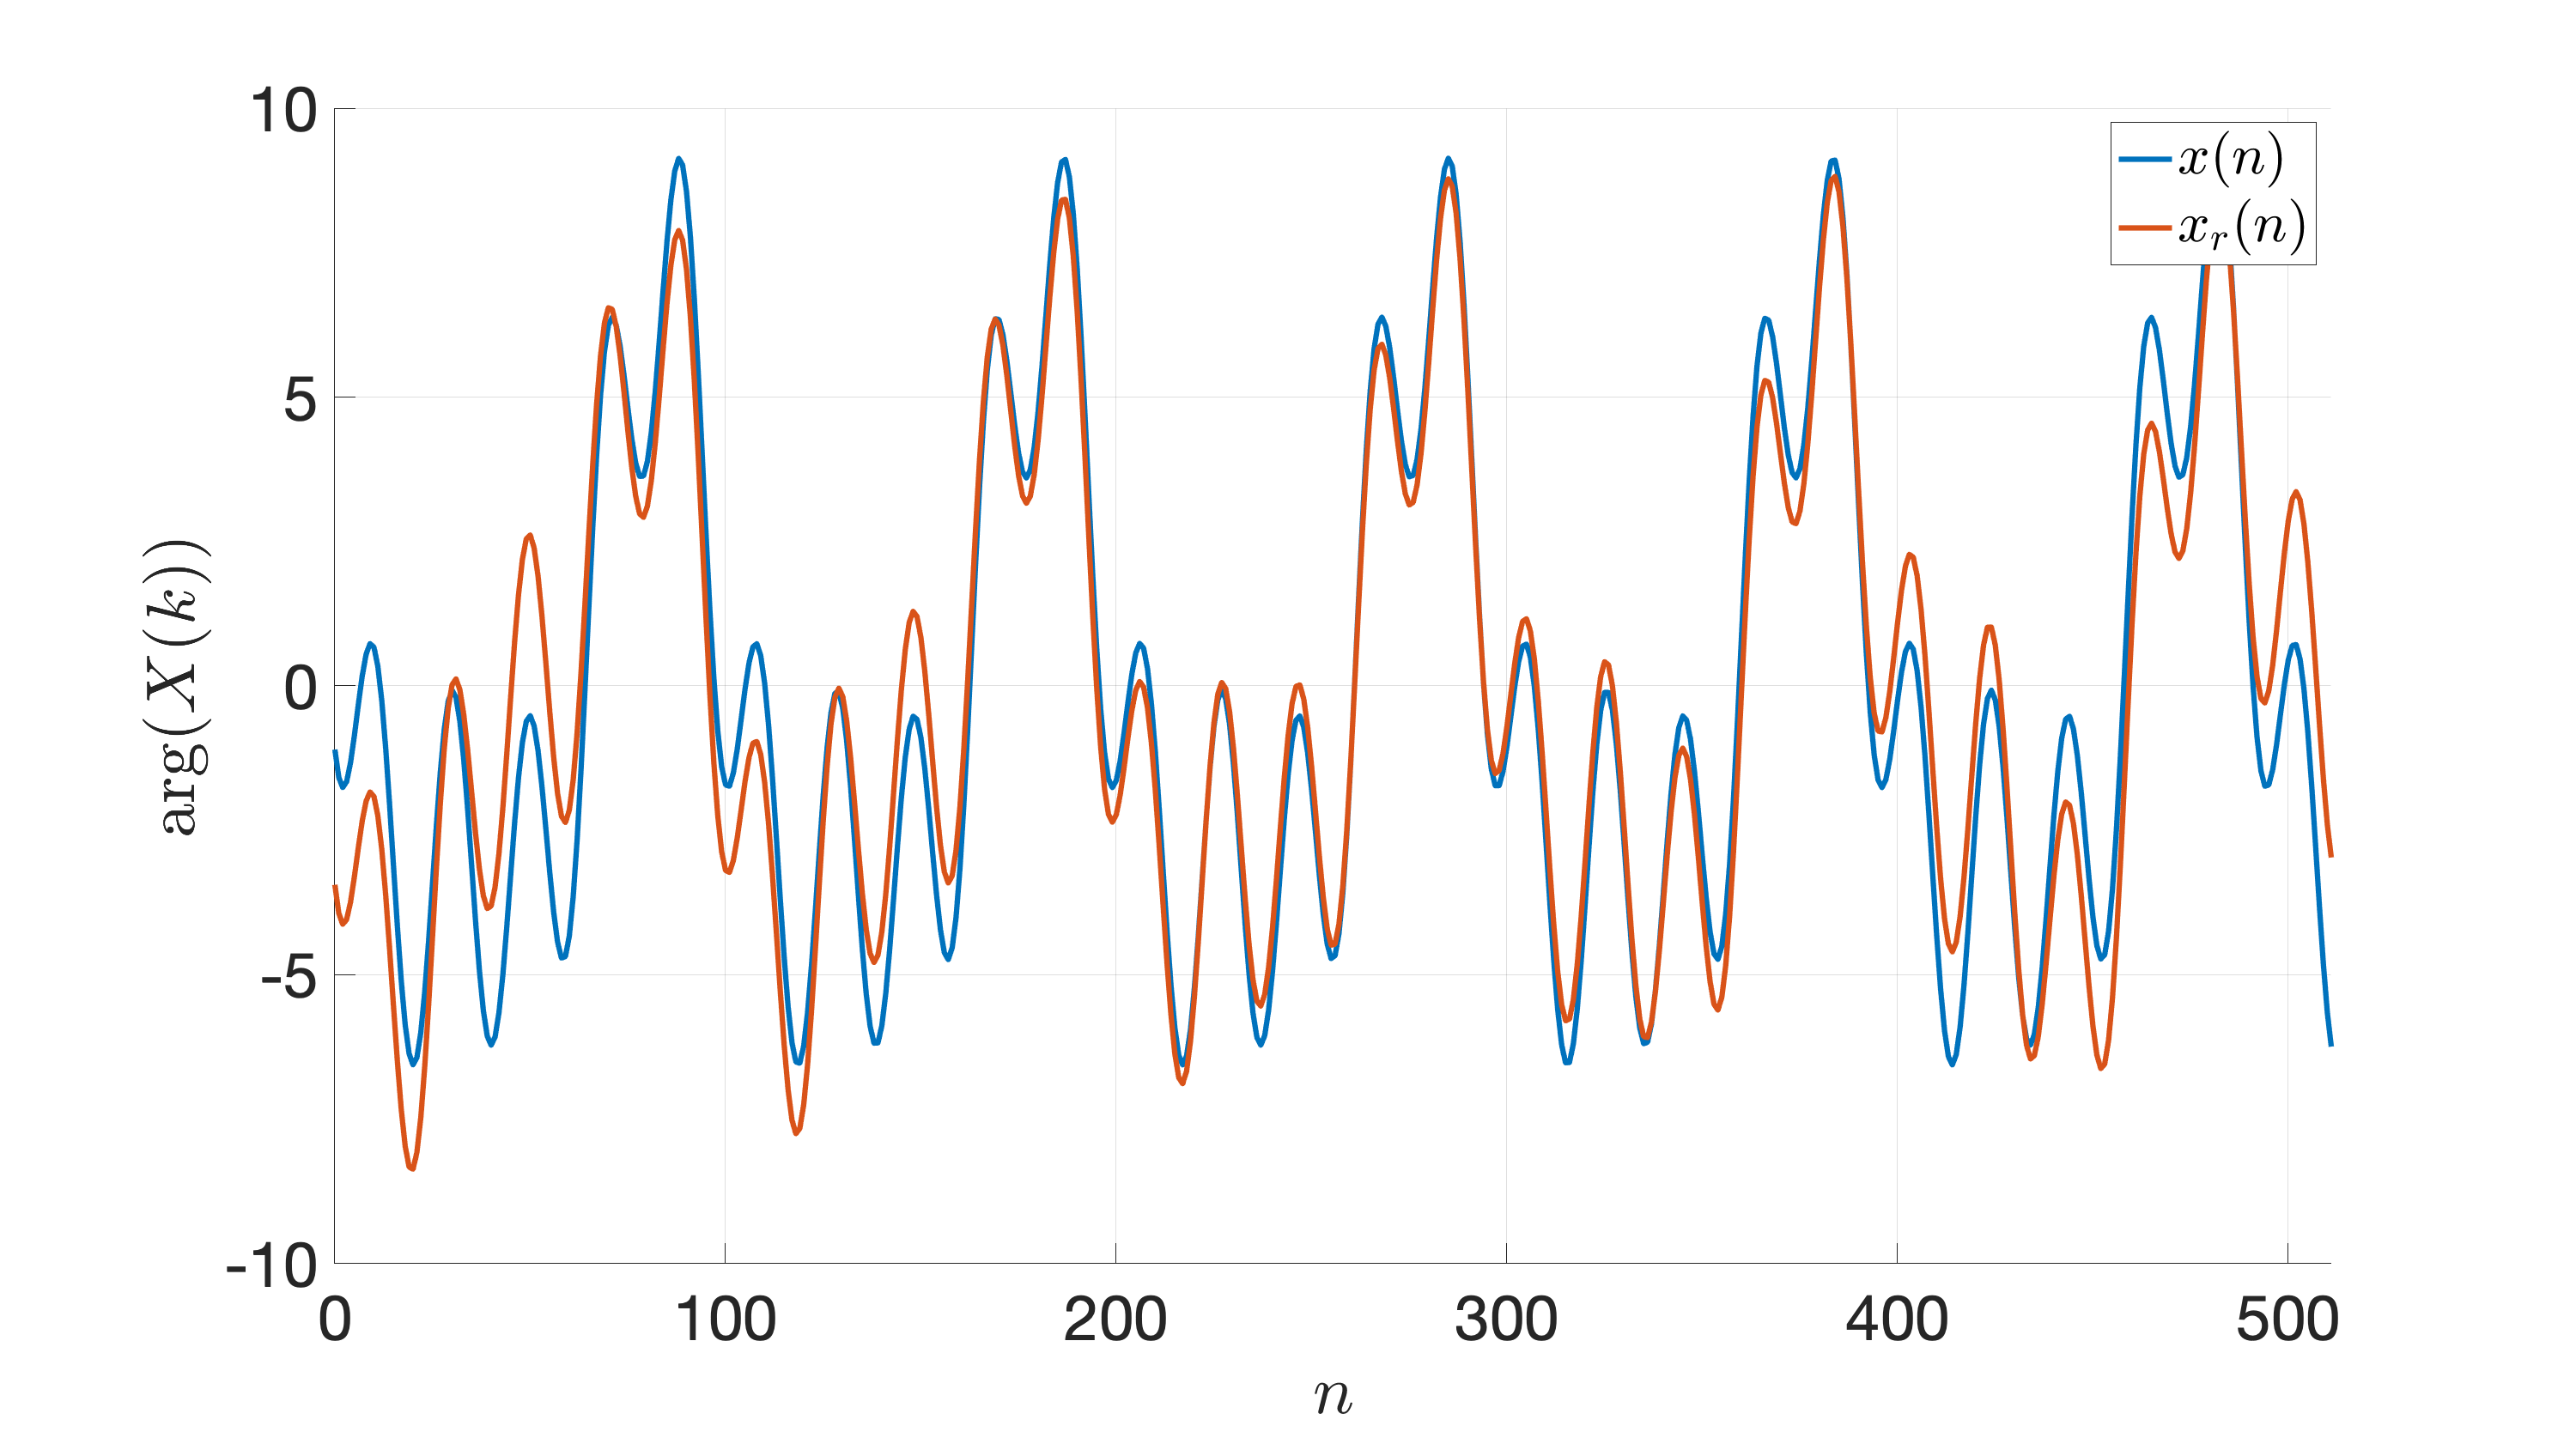
\includegraphics[width= 0.8\textwidth]{figures/R1f.png}
	\caption{Comparison between the reconstructed signal and the original, for $N = 1024$.}
	\label{fig:R1f}
\end{figure}

Furthermore, as pointed out in Section \ref{sec:R1a}, the angular frequency of the lowest harmonic can be written as an irreducible rational fraction of $2\pi$ as $\omega_0 = 2\pi \times 13/1280$. Thus, in order to identify the angular frequencies of all the harmonics exactly, a DFT of length $N = 1280$ is required. As a curiosity, such DFT was performed and the reconstructed signal from the three highest peaks in the one-sided magnitude spectrum is presented in Fig. \ref{fig:R1f_1280}. It is visible that it is able to reproduce the original signal very accurately in the time-domain, achieving $SSE \approx 11.6$.

\begin{figure}[htbp]
	\centering
	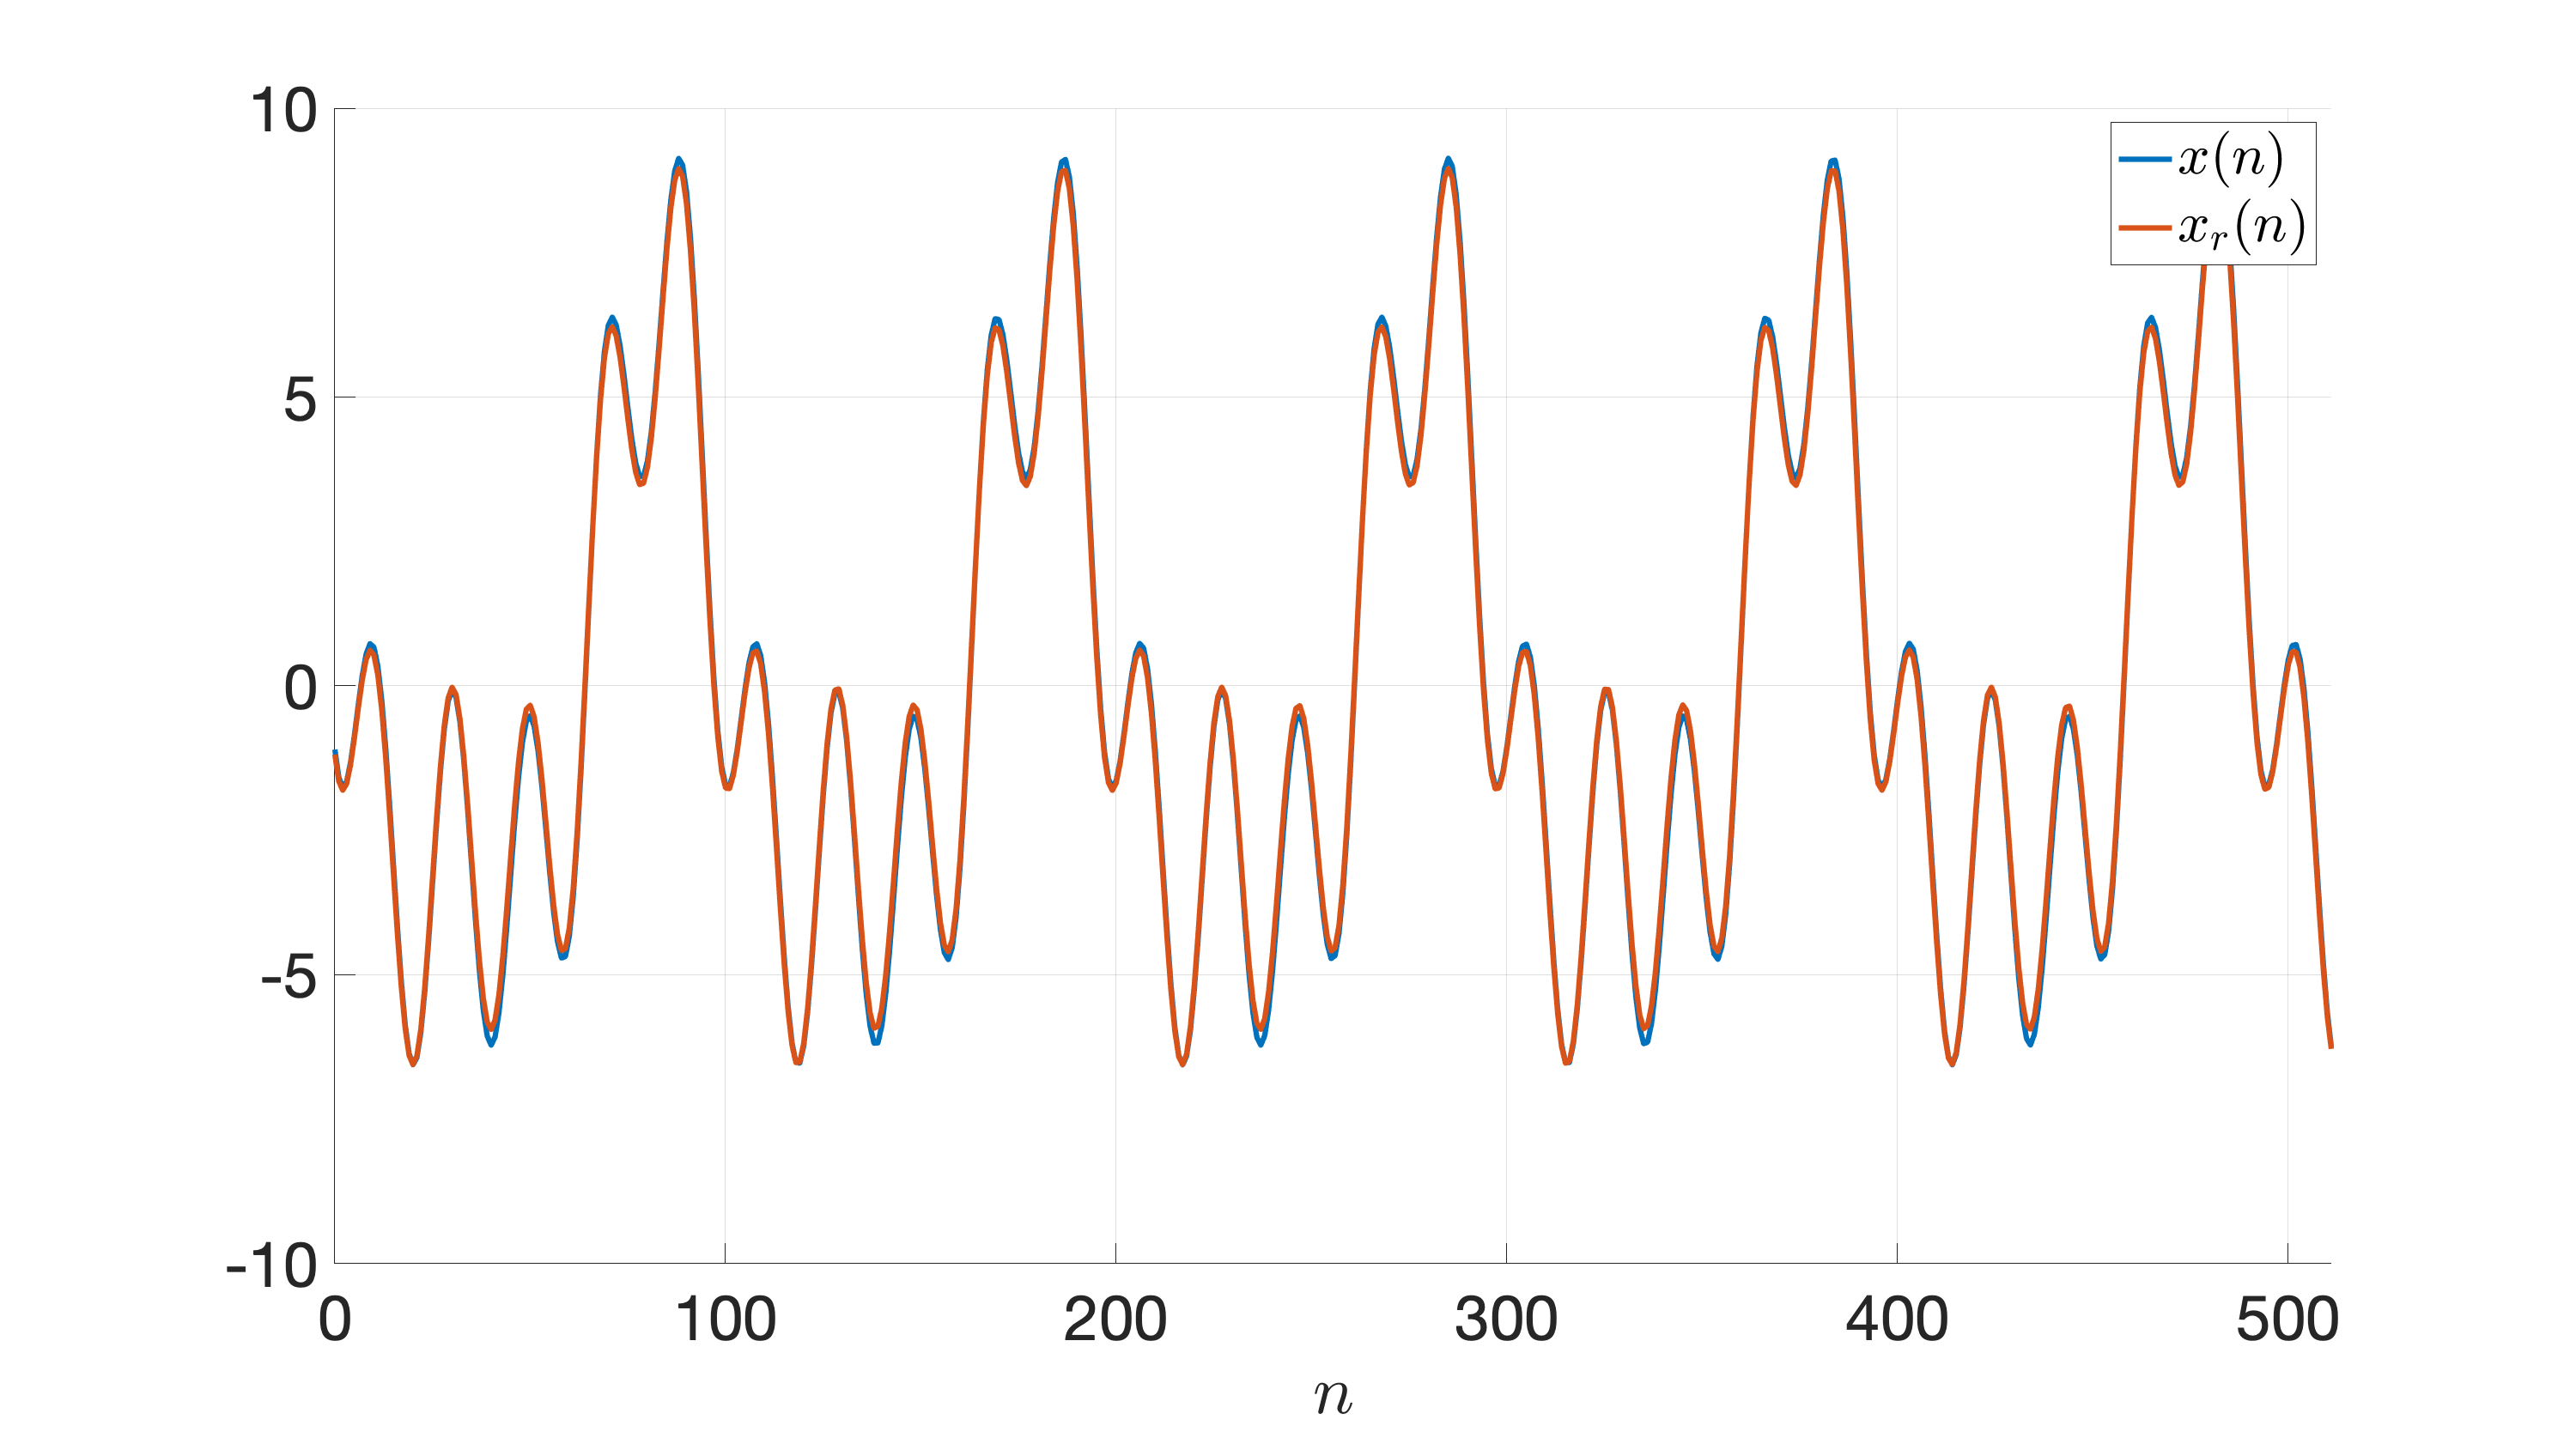
\includegraphics[width= 0.8\textwidth]{figures/R1f_1280.png}
	\caption{Comparison between the reconstructed signal and the original, for $N = 1280$.}
	\label{fig:R1f_1280}
\end{figure}



\end{document}
